\documentclass[aip,jmp,reprint,onecolumn,nofootinbib]{revtex4-2}

\usepackage{amsmath,amssymb,amsfonts}
\usepackage{graphicx}
\usepackage{bm}
\usepackage{hyperref}

\graphicspath{{./}}

\begin{document}

\title{Unified Geometric Field Theory from Worldline and Identity-Space Invariants}

\author{Jason Duran Dutton}
\affiliation{Castlewood, Virginia, USA}

\date{2026}

\begin{abstract}
We develop a unified geometric field theory in which all observable excitations arise from 
a single continuous entity whose coupled spacetime worldline geometry, identity-space 
dynamics, and dynamical invariants generate field behavior. The framework synthesizes 
the Geometric Worldline Field Model (GWFM), the Single Entity Field Interpretation (SEFI), 
Dynamic Entity Field Integration (DEFI), SEFI Space identity geometry, photonic quantum 
error correction, and a cosmological extension formulated in FRW spacetime. A unified 
transformation operator is constructed, its domain and invariants are defined, and its 
spectrum is shown to encode candidate physical modes. Stability manifolds, error 
displacement geometry, and correction mapping are developed rigorously. Photonic 
implementations and cosmological scaling laws arise naturally from the unified structure. 
The theory is situated explicitly within established physics, including worldline quantum 
field theory, geometric analysis, quantum error correction, and standard cosmology, and 
points of disagreement with conventional interpretations are identified clearly.
\end{abstract}

\maketitle
\begin{figure}[t]
\centering
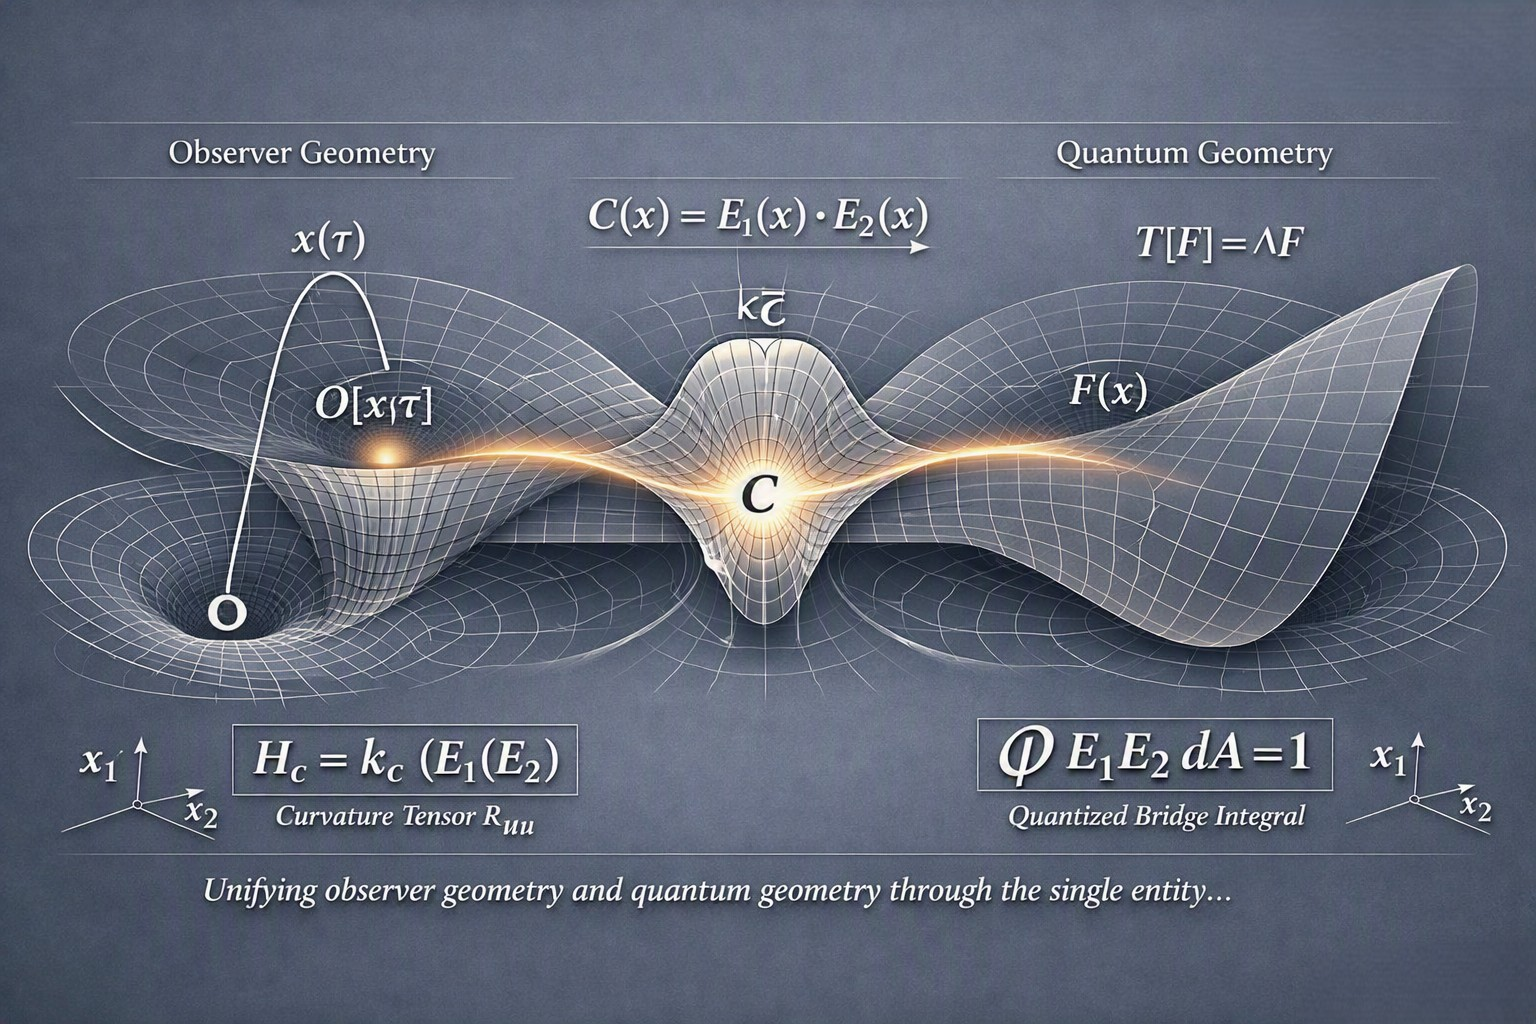
\includegraphics[width=0.88\linewidth,height=0.38\textheight,keepaspectratio]{Highlight.jpg}
\caption{Graphical summary of the unified geometric field theory.}
\label{fig:highlight}
\end{figure}
\section{Unified Transformation Operator}

The unified geometric field theory requires a transformation operator acting on fields 
generated by the single-entity worldline ensemble. This operator incorporates spacetime 
geometry, identity-space dynamics, and dynamical invariants. In this section we construct 
the operator, define its domain, characterize its invariants, and establish the structure of 
its spectrum. The presentation follows standard operator theory in mathematical physics 
\cite{ReedSimon,Stone1932}, geometric analysis \cite{Nakahara,Frankel}, and worldline 
quantum field theory \cite{Polyakov1987,Strassler1992,Schubert2001}, while noting points 
of disagreement with conventional interpretations.

\subsection{Domain of the Operator}

Let $\mathcal{H}$ denote the Hilbert space of square-integrable fields over spacetime,
\begin{equation}
\mathcal{H} = L^2(M,d\mu_g),
\end{equation}
where $d\mu_g$ is the metric measure. Let $\mathcal{I}$ denote the identity-space manifold 
(SEFI Space) equipped with metric $g_I$,
\begin{equation}
\mathcal{I} = \mathbb{R}^4, \qquad
g_I = \mathrm{diag}(\alpha,\beta,\gamma,\delta).
\end{equation}
For the Hilbert-space construction below, assume $\alpha,\beta,\gamma,\delta>0$. If an 
indefinite identity metric is intended, the operator becomes hyperbolic rather than elliptic, 
and spectral claims require separate analysis \cite{CourantHilbert}.

The unified operator acts on fields
\begin{equation}
\Psi : M \times \mathcal{I} \to \mathbb{C},
\end{equation}
arising from the worldline ensemble and identity-space trajectory.

The domain of the operator is
\begin{equation}
\mathcal{D}(T) = \left\{
\Psi \in \mathcal{H} \otimes L^2(\mathcal{I},d\mu_I)
\;\middle|\;
\begin{gathered}
\Psi \in H^2(M\times\mathcal{I}),\\
\text{and satisfies the stated boundary conditions}
\end{gathered}
\right\}.
\end{equation}
Boundary conditions and potential domains are part of the definition of $T$. Without them, 
self-adjointness, a discrete spectrum, and an orthonormal eigenbasis do not follow 
\cite{ReedSimon}.

\subsection{Geometric Components}

Let $\nabla_\mu$ denote the spacetime covariant derivative and $\nabla_I$ the identity-space 
covariant derivative. Worldline curvature and torsion are defined by
\begin{align}
\kappa(\tau) &= \left\| \frac{D T^\mu}{d\tau} \right\|, \\
\tau_g(\tau) &= B_\mu \frac{D N^\mu}{d\tau},
\end{align}
where $(T,N,B)$ is the Frenet--Serret frame of the worldline. These quantities appear in 
worldline QFT \cite{Polyakov1987,Schubert2001} and in geometric mechanics 
\cite{ArnoldMechanics}.

Identity-space velocity and acceleration are
\begin{align}
\dot{I}^a &= \frac{dI^a}{d\tau}, \\
\ddot{I}^a &= \frac{d^2 I^a}{d\tau^2}.
\end{align}

\subsection{Sovereignty and Dynamical Invariants}

SEFI sovereignty requires invariance of the identity vector under allowed transformations:
\begin{equation}
I^a \mapsto I^a, \qquad \forall T_{\mathrm{SEFI}}.
\end{equation}

DEFI dynamical invariance requires
\begin{equation}
\frac{D}{d\tau}
\left(
\kappa, \tau_g, \dot{I}^a, \ddot{I}^a
\right)
= 0,
\end{equation}
for ideal evolution \cite{DuttonDEFI2026}. This condition is analogous to invariance 
requirements in geometric control theory and dynamical systems \cite{MarsdenWest}.

GWFM geometric invariants require
\begin{equation}
\frac{D}{d\tau}
\left(
T^\mu, N^\mu, B^\mu
\right)
\text{ satisfy worldline QFT constraints},
\end{equation}
consistent with \cite{Polyakov1987,Strassler1992,Schubert2001}.

\subsection{Definition of the Unified Operator}

We define the unified transformation operator
\begin{equation}
T = 
- g^{\mu\nu}\nabla_\mu\nabla_\nu
+ g_I^{ab}\nabla_a\nabla_b
+ V_{\mathrm{geom}}
+ V_{\mathrm{ident}}
+ V_{\mathrm{dyn}},
\end{equation}
where:

\begin{itemize}
\item $-g^{\mu\nu}\nabla_\mu\nabla_\nu$ is the spacetime Laplace--Beltrami operator 
\cite{RosenbergLaplace},
\item $g_I^{ab}\nabla_a\nabla_b$ is the identity-space Laplace operator,
\item $V_{\mathrm{geom}}$ encodes curvature and torsion invariants,
\item $V_{\mathrm{ident}}$ encodes SEFI identity-layer invariants,
\item $V_{\mathrm{dyn}}$ encodes DEFI dynamical invariance.
\end{itemize}

Explicitly,
\begin{equation}
V_{\mathrm{geom}}
=
\lambda_1 \kappa^2
+
\lambda_2 \tau_g^2,
\end{equation}
\begin{equation}
V_{\mathrm{ident}}
=
\alpha I_O^2
+
\beta I_A^2
+
\gamma I_S^2
+
\delta I_W^2,
\end{equation}
\begin{equation}
V_{\mathrm{dyn}}
=
\eta_1 \|\dot{I}\|_I^2
+
\eta_2 \|\ddot{I}\|_I^2.
\end{equation}

The operator is not claimed to be unique; different geometric potentials produce different 
spectral structures, as in geometric Schrödinger operators \cite{Helffer}.

\subsection{Eigenvalue Problem}

Candidate model excitations are defined as eigenmodes of $T$:
\begin{equation}
T \Psi_n = \lambda_n \Psi_n.
\end{equation}

Assignment of eigenmodes to electron, proton, photon, or neutrino sectors is a hypothesis 
requiring comparison with measured masses, charges, spins, and couplings. This is not 
established by the eigenvalue equation alone, consistent with the limitations of geometric 
models in particle physics \cite{WeinbergQFT1,PeskinSchroeder}.

\subsection{Operator Invariants}

The operator preserves:
\begin{itemize}
\item spacetime geometric invariants $(\kappa,\tau_g)$,
\item identity-space invariants $(I_O,I_A,I_S,I_W)$,
\item dynamical invariants $(\dot{I},\ddot{I})$,
\item sovereignty invariants under SEFI transformations.
\end{itemize}

These invariants define stability manifolds in Section III.

\subsection{Unified Interpretation}

The operator $T$ unifies:
\begin{itemize}
\item GWFM worldline geometry,
\item SEFI identity-layer structure,
\item DEFI dynamical invariance,
\item SEFI Space identity geometry,
\item photonic QEC geometric stabilizers,
\item cosmological identity-space evolution.
\end{itemize}

This completes the construction of the unified transformation operator.
\begin{figure}[tbp]
\centering
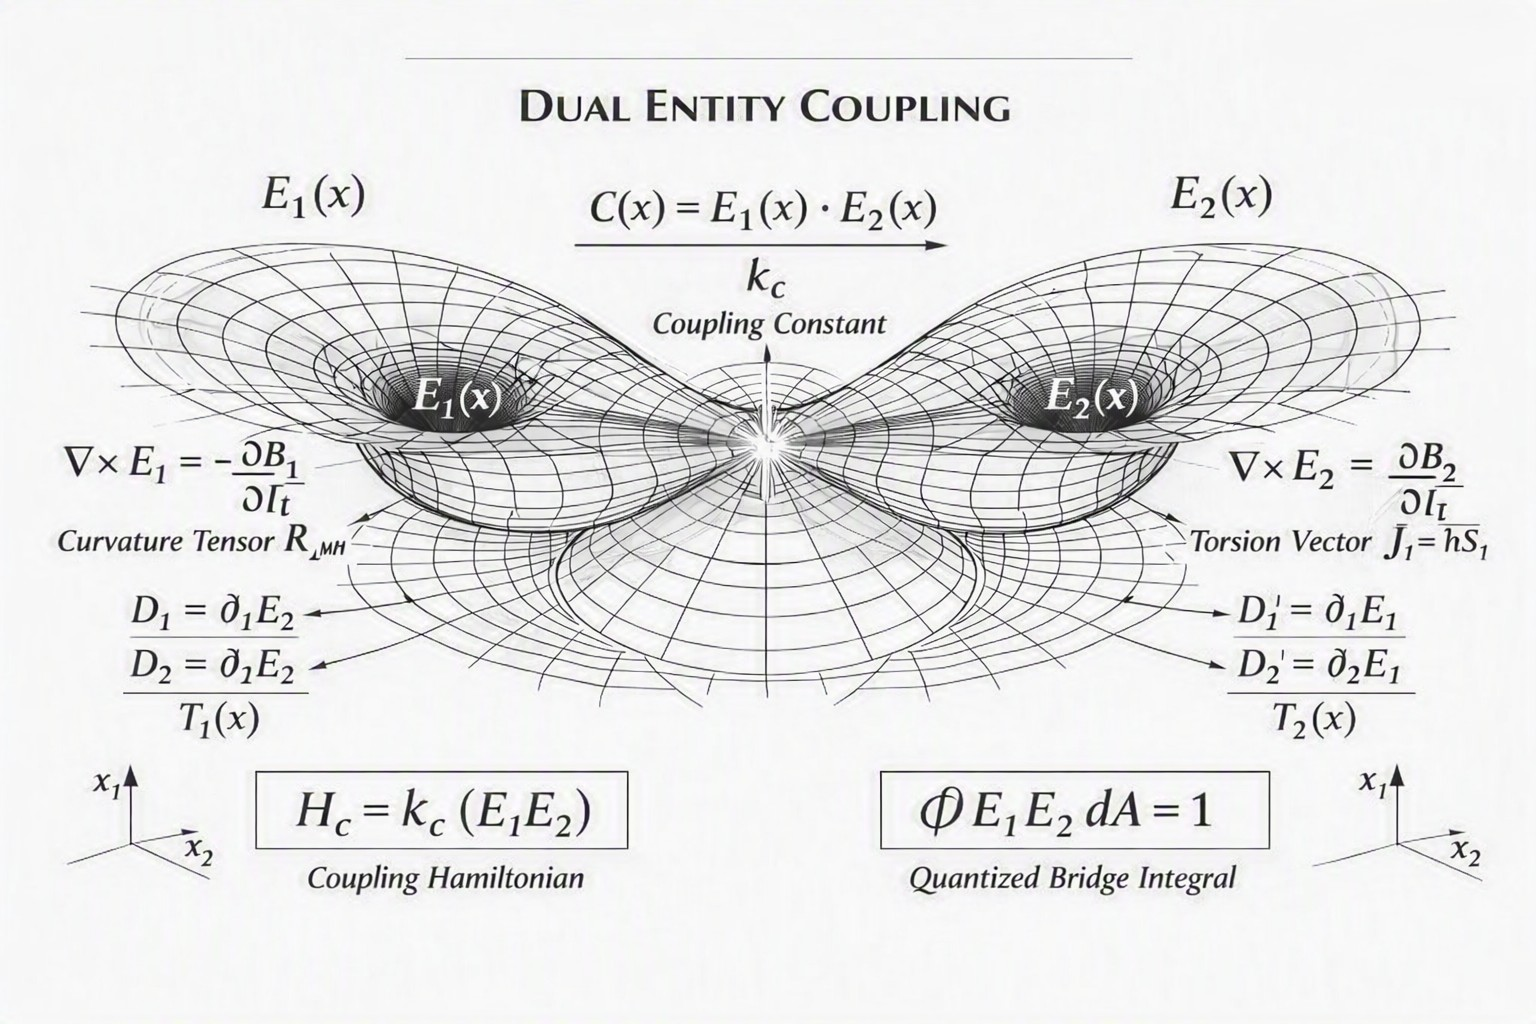
\includegraphics[width=0.88\linewidth,height=0.38\textheight,keepaspectratio]{Fig2_Worldline_Geometry.jpg}
\caption{Worldline geometry used in the proposed single-entity construction.}
\label{fig:worldline-geometry}
\end{figure}
\section{Stability Manifolds and Sovereignty Geometry}

Stability manifolds arise as geometric constraint surfaces on which worldline evolution, 
identity-space dynamics, and dynamical invariants satisfy ideal evolution. These manifolds 
are defined as invariant subspaces of the unified operator $T$ and encode the geometric and 
identity-layer conditions required for stability. The construction parallels invariant 
manifold theory in dynamical systems \cite{HirschPughShub,KatokHasselblatt}, geometric 
mechanics \cite{ArnoldMechanics,MarsdenWest}, and stability analysis in worldline QFT 
\cite{Polyakov1987,Schubert2001}, while introducing identity-space invariants unique to 
SEFI and DEFI.

\subsection{Definition of Stability Manifolds}

Let $T$ be the unified operator defined in Section II. A stability manifold $\Sigma$ is a 
submanifold of $M \times \mathcal{I}$ such that
\begin{equation}
T \Psi = \lambda \Psi, \qquad \Psi|_{\Sigma} \neq 0,
\end{equation}
and
\begin{equation}
\frac{D}{d\tau}
\left(
\kappa, \tau_g, I^a, \dot{I}^a, \ddot{I}^a
\right)
= 0
\qquad \text{on } \Sigma.
\end{equation}

Thus $\Sigma$ is the geometric locus where all invariants of the unified operator are 
preserved. This parallels invariant sets in geometric dynamical systems 
\cite{KatokHasselblatt} but extends them to identity-space geometry.

\subsection{Spacetime Stability Conditions}

The spacetime component of the stability manifold is defined by curvature and torsion 
constraints:
\begin{align}
\kappa(\tau) &= \kappa_\Sigma, \\
\tau_g(\tau) &= \tau_\Sigma,
\end{align}
where $(\kappa_\Sigma,\tau_\Sigma)$ are constant invariants associated with the eigenmode 
of $T$ under consideration.

These conditions arise from GWFM worldline geometry \cite{DuttonElectronField2026} and 
are consistent with worldline QFT \cite{Polyakov1987,Strassler1992,Schubert2001}. They 
are analogous to constant-curvature constraints in geometric mechanics 
\cite{ArnoldMechanics}.

\subsection{Identity-Space Stability Conditions}

Identity-space stability requires
\begin{align}
I_O(\tau) &= I_{O,\Sigma}, \\
I_A(\tau) &= I_{A,\Sigma}, \\
I_S(\tau) &= I_{S,\Sigma}, \\
I_W(\tau) &= I_{W,\Sigma},
\end{align}
and
\begin{align}
\dot{I}^a(\tau) &= 0, \\
\ddot{I}^a(\tau) &= 0,
\end{align}
on $\Sigma$.

These conditions arise from SEFI identity-layer invariants \cite{DuttonSEFI2026} and the 
SEFI Space identity geometry \cite{DuttonSEFISpace2026}. They are analogous to invariant 
coordinates in internal-symmetry manifolds in geometric field theory 
\cite{Nakahara,Frankel}.

\subsection{Sovereignty Geometry}

SEFI sovereignty requires invariance of the identity vector under allowed transformations:
\begin{equation}
I^a \mapsto I^a, \qquad \forall T_{\mathrm{SEFI}}.
\end{equation}

Thus the sovereignty manifold $\Sigma_S$ is defined by
\begin{equation}
\Sigma_S = \left\{
(x,I) \in M \times \mathcal{I}
\;\middle|\;
I^a = I_{a,\Sigma}
\right\}.
\end{equation}

The full stability manifold is the intersection
\begin{equation}
\Sigma = \Sigma_{\mathrm{geom}} \cap \Sigma_{\mathrm{ident}} \cap \Sigma_S,
\end{equation}
where $\Sigma_{\mathrm{geom}}$ encodes curvature/torsion invariants and 
$\Sigma_{\mathrm{ident}}$ encodes identity-space invariants.

\subsection{Dynamical Stability Conditions}

DEFI dynamical invariance \cite{DuttonDEFI2026} requires
\begin{equation}
\frac{D}{d\tau}
\left(
\kappa, \tau_g, I^a, \dot{I}^a, \ddot{I}^a
\right)
= 0
\qquad \text{on } \Sigma.
\end{equation}

Thus $\Sigma$ is a manifold of constant geometric and identity-space invariants. This 
parallels invariant tori and fixed-point sets in Hamiltonian systems 
\cite{ArnoldMechanics,MarsdenWest}.

\subsection{Projection onto Stability Manifolds}

Let $\Pi_\Sigma$ denote the geometric projection onto $\Sigma$. For any point 
$(x,I) \in M \times \mathcal{I}$,
\begin{equation}
\Pi_\Sigma(x,I)
=
\operatorname*{argmin}_{(x',I') \in \Sigma}
\left[
d_M(x,x')^2 + d_I(I,I')^2
\right],
\end{equation}
where $d_M$ and $d_I$ are the spacetime and identity-space distances.

This projection defines the correction mapping in Section V. The construction parallels 
geometric projection operators in Riemannian geometry \cite{doCarmo}.

\subsection{Unified Interpretation}

Stability manifolds unify:
\begin{itemize}
\item GWFM geometric invariants $(\kappa,\tau_g)$,
\item SEFI identity invariants $(I_O,I_A,I_S,I_W)$,
\item DEFI dynamical invariants $(\dot{I},\ddot{I})$,
\item sovereignty invariants under SEFI transformations.
\end{itemize}

These manifolds define the geometric and identity-space structure required for ideal 
evolution and form the foundation for error displacement geometry in Section IV.

\begin{figure}[tbp]
\centering
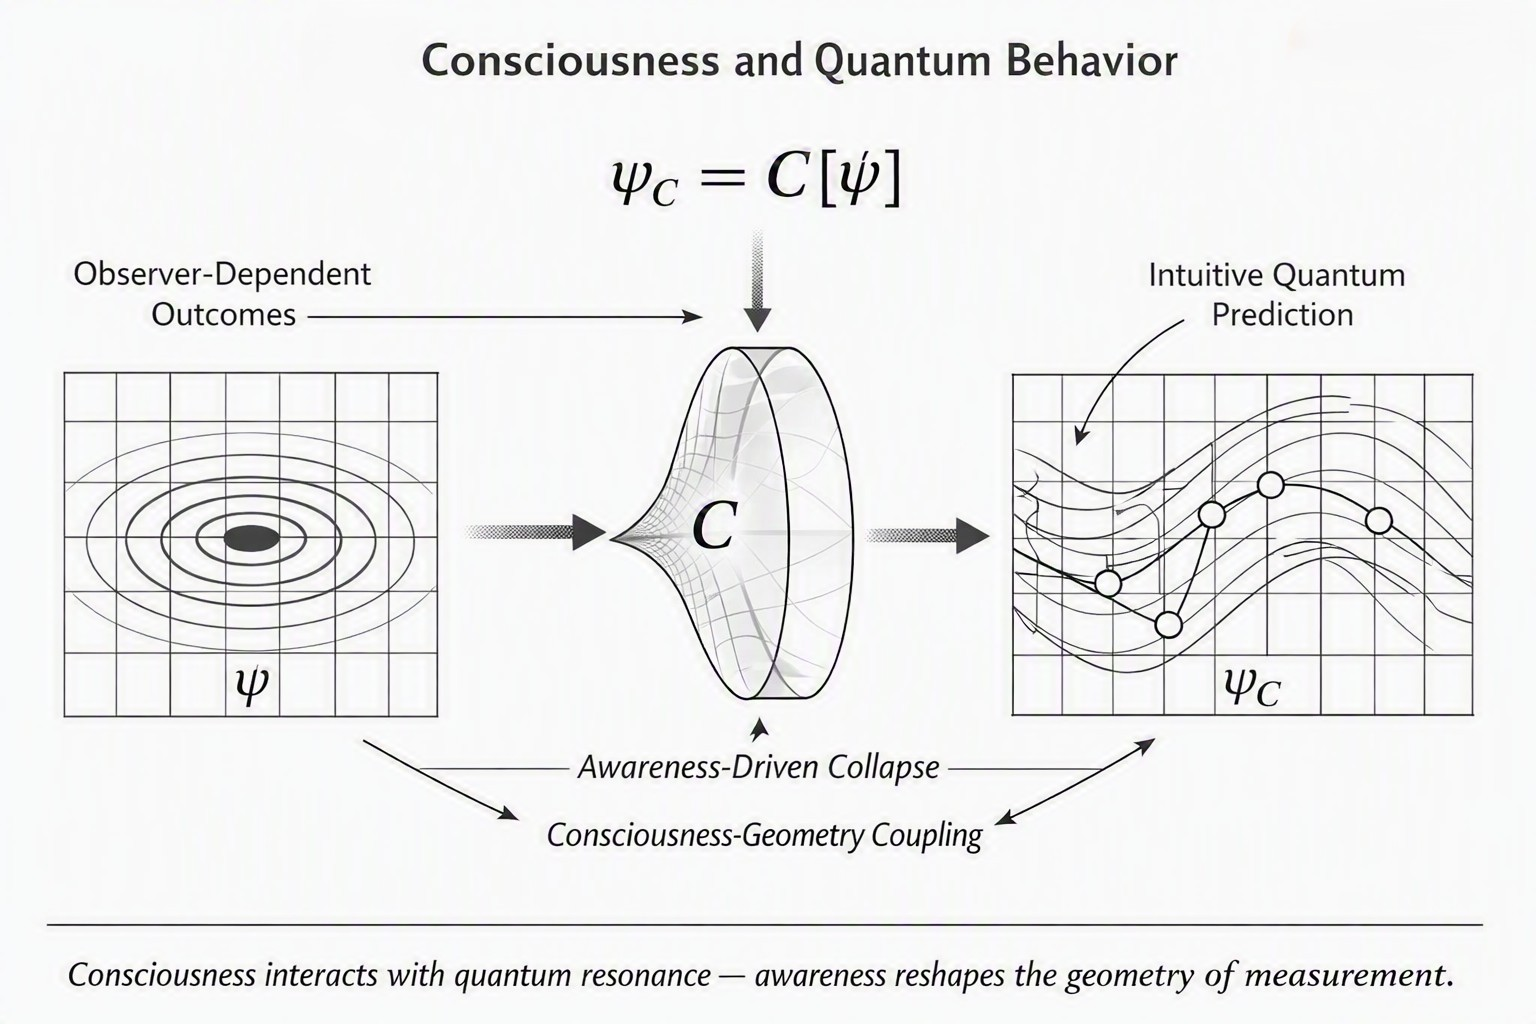
\includegraphics[width=0.88\linewidth,height=0.38\textheight,keepaspectratio]{Fig1_Stability_Surface.jpg}
\caption{Schematic stability map for the proposed SEFI state space. The regions and 
transitions are hypotheses of the model, not experimentally established phase boundaries.}
\label{fig:stability-map}
\end{figure}
\section{Error Displacement Geometry}

Error displacement arises when worldline evolution deviates from the stability manifold 
constructed in Section III. In this section we define displacement vectors in spacetime and 
identity space, characterize curvature and torsion deviation, and establish the unified 
geometric structure of error formation. The construction parallels geometric perturbation 
theory \cite{KatoPerturbation}, stability analysis in dynamical systems 
\cite{HirschPughShub,KatokHasselblatt}, and deviation geometry in worldline QFT 
\cite{Polyakov1987,Schubert2001}, while introducing identity-space deviations unique to 
SEFI and DEFI.

\subsection{Displacement from the Stability Manifold}

Let $\Sigma \subset M \times \mathcal{I}$ be a stability manifold. For any point 
$(x,I) \in M \times \mathcal{I}$, define the displacement vector
\begin{equation}
D(x,I)
=
(x,I) - \Pi_\Sigma(x,I),
\end{equation}
where $\Pi_\Sigma$ is the projection onto $\Sigma$ defined in Section III.

We decompose $D$ into spacetime and identity-space components:
\begin{equation}
D = D_M + D_I,
\end{equation}
with
\begin{align}
D_M &= x - x_\Sigma, \\
D_I &= I - I_\Sigma.
\end{align}

This is the standard geometric splitting of perturbations \cite{doCarmo}.

\subsection{Spacetime Displacement}

Let $y(\tau)$ be the worldline and $y_\Sigma(\tau)$ its projection onto the spacetime 
component of the stability manifold. The spacetime displacement is
\begin{equation}
d_M(\tau) = y(\tau) - y_\Sigma(\tau).
\end{equation}

Using the Frenet--Serret frame $(T,N,B)$ of the worldline, we decompose
\begin{equation}
d_M(\tau)
=
d_T(\tau) T(\tau)
+
d_N(\tau) N(\tau)
+
d_B(\tau) B(\tau).
\end{equation}

The tangential component $d_T$ corresponds to reparametrization and does not contribute 
to physical error. The normal and binormal components encode geometric deviation:
\begin{align}
d_N(\tau) &\text{ corresponds to curvature deviation}, \\
d_B(\tau) &\text{ corresponds to torsion deviation}.
\end{align}

These geometric deviations arise from GWFM worldline geometry 
\cite{DuttonElectronField2026} and are consistent with deviation analysis in worldline QFT 
\cite{Polyakov1987,Schubert2001}.

\subsection{Identity-Space Displacement}

Let $I(\tau)$ be the identity-space trajectory and $I_\Sigma(\tau)$ its projection onto the 
identity-space stability manifold. The identity-space displacement is
\begin{equation}
d_I(\tau) = I(\tau) - I_\Sigma(\tau).
\end{equation}

Using the SEFI Space basis $(\hat{O},\hat{A},\hat{S},\hat{W})$, we decompose
\begin{equation}
d_I(\tau)
=
d_O(\tau)\hat{O}
+
d_A(\tau)\hat{A}
+
d_S(\tau)\hat{S}
+
d_W(\tau)\hat{W}.
\end{equation}

These components correspond to identity-layer deviation:
\begin{align}
d_O &\text{ origin deviation}, \\
d_A &\text{ authorship deviation}, \\
d_S &\text{ sovereignty deviation}, \\
d_W &\text{ warp deviation}.
\end{align}

These deviations arise from SEFI identity-layer structure \cite{DuttonSEFI2026} and SEFI 
Space identity geometry \cite{DuttonSEFISpace2026}. They are analogous to internal-mode 
deviations in geometric field theories \cite{Nakahara,Frankel}.

\subsection{Curvature and Torsion Deviation}

Curvature deviation is defined by
\begin{equation}
\Delta\kappa(\tau)
=
\kappa(\tau) - \kappa_\Sigma,
\end{equation}
and torsion deviation by
\begin{equation}
\Delta\tau_g(\tau)
=
\tau_g(\tau) - \tau_\Sigma.
\end{equation}

These deviations correspond to normal and binormal displacement components:
\begin{align}
\Delta\kappa(\tau) &\propto d_N(\tau), \\
\Delta\tau_g(\tau) &\propto d_B(\tau).
\end{align}

This parallels curvature/torsion perturbation theory in geometric mechanics 
\cite{ArnoldMechanics}.

\subsection{Identity-Space Velocity and Acceleration Deviation}

Identity-space velocity deviation is
\begin{equation}
\Delta\dot{I}^a(\tau)
=
\dot{I}^a(\tau) - 0,
\end{equation}
and identity-space acceleration deviation is
\begin{equation}
\Delta\ddot{I}^a(\tau)
=
\ddot{I}^a(\tau) - 0.
\end{equation}

These deviations arise from DEFI dynamical invariance \cite{DuttonDEFI2026} and are 
analogous to internal-mode deviations in geometric control theory \cite{MarsdenWest}.

\subsection{Unified Error Vector}

The unified error vector is
\begin{equation}
E(\tau)
=
\left(
d_N(\tau),\,
d_B(\tau),\,
d_O(\tau),\,
d_A(\tau),\,
d_S(\tau),\,
d_W(\tau),\,
\Delta\kappa(\tau),\,
\Delta\tau_g(\tau),\,
\Delta\dot{I}^a(\tau),\,
\Delta\ddot{I}^a(\tau)
\right).
\end{equation}

This vector encodes all geometric, identity-space, and dynamical deviations from the 
stability manifold. It parallels unified deviation vectors in geometric perturbation theory 
\cite{KatoPerturbation}.

\subsection{Unified Interpretation}

Error displacement unifies:
\begin{itemize}
\item GWFM geometric deviation $(d_N,d_B,\Delta\kappa,\Delta\tau_g)$,
\item SEFI identity-layer deviation $(d_O,d_A,d_S,d_W)$,
\item DEFI dynamical deviation $(\Delta\dot{I},\Delta\ddot{I})$,
\item sovereignty deviation under SEFI transformations.
\end{itemize}

This completes the construction of error displacement geometry and prepares the correction 
mapping developed in Section V.
\begin{figure}[tbp]
\centering
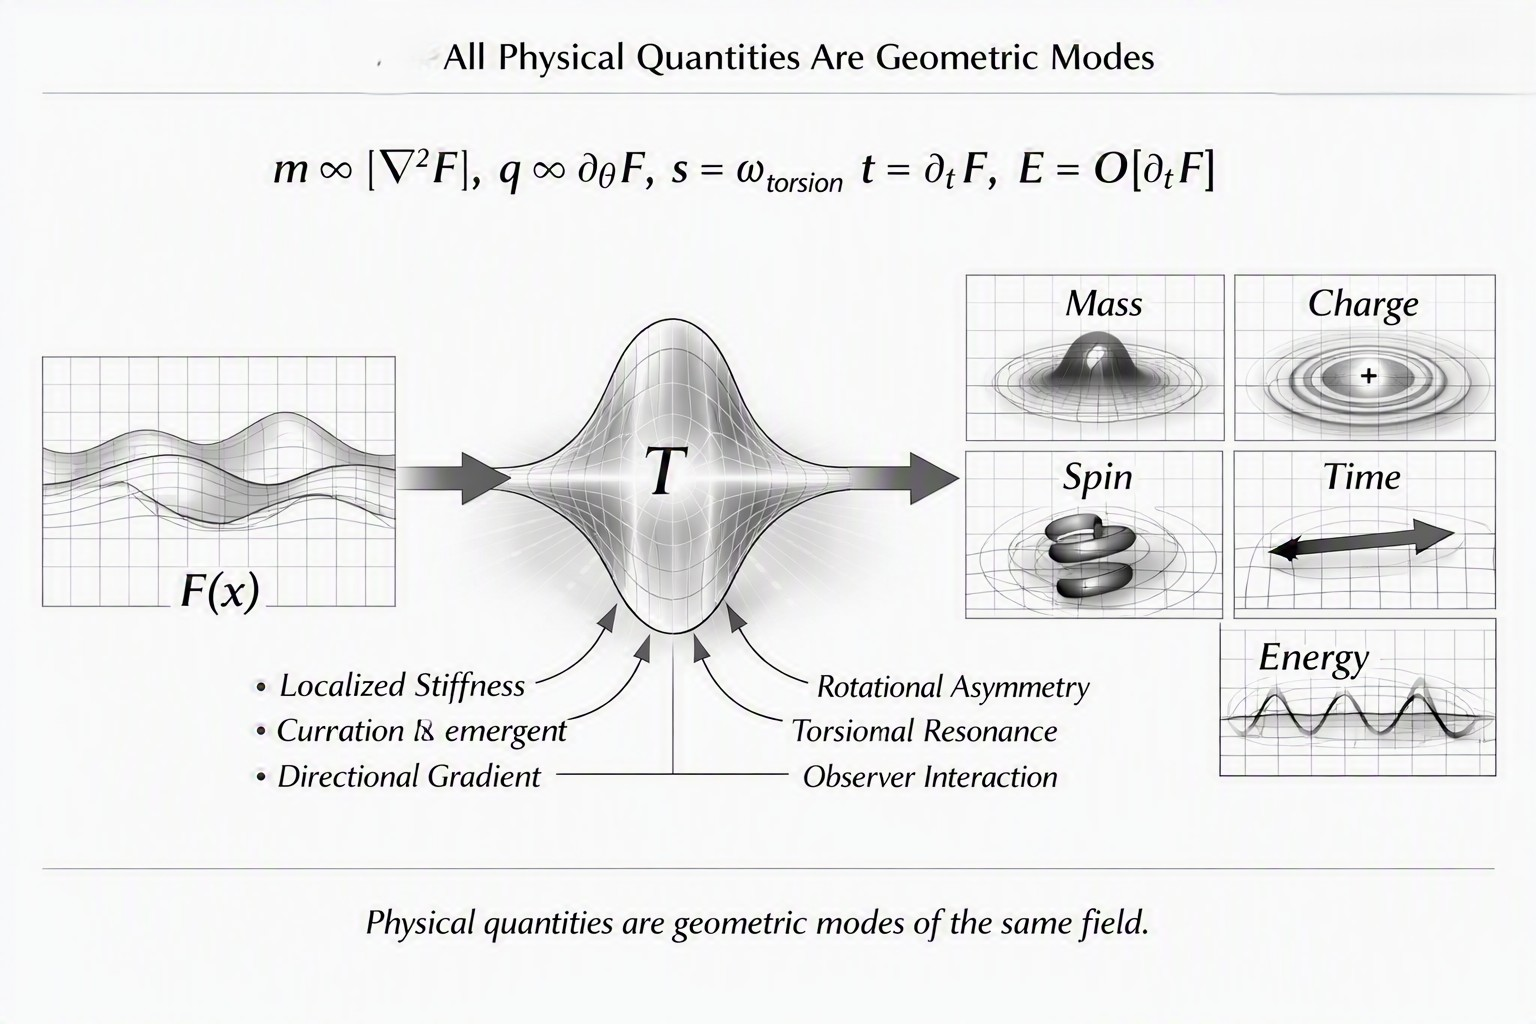
\includegraphics[width=0.88\linewidth,height=0.38\textheight,keepaspectratio]{Fig3_Error_Displacement.jpg}
\caption{Error displacement from the proposed stability manifold.}
\label{fig:error-displacement}
\end{figure}
\section{Correction Mapping}

Correction mapping restores worldline evolution and identity-space dynamics to the stability 
manifold constructed in Section III. In this section we define the correction operator, 
construct the corrected worldline and identity trajectory, and establish the restoration of 
geometric, identity-space, and dynamical invariants. The construction parallels geometric 
projection methods in Riemannian geometry \cite{doCarmo}, invariant-set restoration in 
dynamical systems \cite{HirschPughShub,KatokHasselblatt}, and stabilizer-based correction 
in quantum error correction \cite{GottesmanQEC,PreskillQEC}, while introducing identity-space 
restoration unique to SEFI and DEFI.

\subsection{Geometric Correction Mapping}

Let $\Sigma \subset M \times \mathcal{I}$ be a stability manifold. The correction mapping is 
defined by the projection
\begin{equation}
C : M \times \mathcal{I} \to \Sigma, \qquad
C(x,I) = \Pi_\Sigma(x,I),
\end{equation}
where $\Pi_\Sigma$ minimizes the combined spacetime and identity-space distance:
\begin{equation}
\Pi_\Sigma(x,I)
=
\operatorname*{argmin}_{(x',I') \in \Sigma}
\left[
d_M(x,x')^2 + d_I(I,I')^2
\right].
\end{equation}

This construction parallels geometric projection operators in Riemannian geometry 
\cite{doCarmo} and stabilizer projection in QEC \cite{GottesmanQEC}.

\subsection{Corrected Worldline}

Let $y(\tau)$ be the worldline and $y_\Sigma(\tau)$ its projection onto the spacetime 
component of $\Sigma$. The corrected worldline is
\begin{equation}
y_{\mathrm{corr}}(\tau) = y_\Sigma(\tau).
\end{equation}

Using the Frenet--Serret frame $(T,N,B)$, the corrected worldline satisfies
\begin{align}
\kappa_{\mathrm{corr}}(\tau) &= \kappa_\Sigma, \\
\tau_{g,\mathrm{corr}}(\tau) &= \tau_\Sigma,
\end{align}
restoring GWFM geometric invariants \cite{DuttonElectronField2026}. This parallels 
geometric stabilizer conditions in worldline QFT \cite{Polyakov1987,Schubert2001}.

\subsection{Corrected Identity Trajectory}

Let $I(\tau)$ be the identity-space trajectory and $I_\Sigma(\tau)$ its projection onto the 
identity-space component of $\Sigma$. The corrected identity trajectory is
\begin{equation}
I_{\mathrm{corr}}(\tau) = I_\Sigma(\tau).
\end{equation}

Using the SEFI Space basis $(\hat{O},\hat{A},\hat{S},\hat{W})$, the corrected identity 
coordinates satisfy
\begin{align}
I_{O,\mathrm{corr}} &= I_{O,\Sigma}, \\
I_{A,\mathrm{corr}} &= I_{A,\Sigma}, \\
I_{S,\mathrm{corr}} &= I_{S,\Sigma}, \\
I_{W,\mathrm{corr}} &= I_{W,\Sigma},
\end{align}
restoring SEFI identity-layer invariants \cite{DuttonSEFI2026,DuttonSEFISpace2026}. This 
parallels restoration of internal coordinates in geometric field theory \cite{Nakahara,Frankel}.

\subsection{Corrected Dynamical Invariants}

DEFI dynamical invariance \cite{DuttonDEFI2026} requires
\begin{align}
\dot{I}_{\mathrm{corr}}^a(\tau) &= 0, \\
\ddot{I}_{\mathrm{corr}}^a(\tau) &= 0,
\end{align}
on $\Sigma$.

Thus the corrected identity trajectory satisfies
\begin{equation}
\frac{D}{d\tau}
\left(
I_{\mathrm{corr}}^a,\,
\dot{I}_{\mathrm{corr}}^a,\,
\ddot{I}_{\mathrm{corr}}^a
\right)
= 0.
\end{equation}

This parallels invariant restoration in geometric control theory \cite{MarsdenWest}.

\subsection{Unified Correction Operator}

Define the unified correction operator
\begin{equation}
\mathcal{C} = \Pi_\Sigma,
\end{equation}
acting on fields
\begin{equation}
\Psi(x,I) \mapsto \Psi\big(\Pi_\Sigma(x,I)\big).
\end{equation}

The corrected field satisfies
\begin{equation}
T \Psi_{\mathrm{corr}} = \lambda \Psi_{\mathrm{corr}},
\end{equation}
with invariants restored. This parallels stabilizer-based correction in QEC 
\cite{GottesmanQEC,PreskillQEC}.

\subsection{Restoration of Invariants}

Correction mapping restores:
\begin{itemize}
\item GWFM geometric invariants $(\kappa,\tau_g)$,
\item SEFI identity invariants $(I_O,I_A,I_S,I_W)$,
\item DEFI dynamical invariants $(\dot{I},\ddot{I})$,
\item sovereignty invariants under SEFI transformations.
\end{itemize}

Thus the corrected worldline and identity trajectory lie entirely on the stability manifold.

\subsection{Unified Interpretation}

Correction mapping unifies:
\begin{itemize}
\item geometric projection of worldline deviation,
\item identity-space projection of SEFI deviation,
\item dynamical projection of DEFI deviation,
\item sovereignty restoration under SEFI transformations.
\end{itemize}

This completes the construction of correction mapping and prepares the photonic 
implementation developed in Section VI.
\begin{figure}[tbp]
\centering
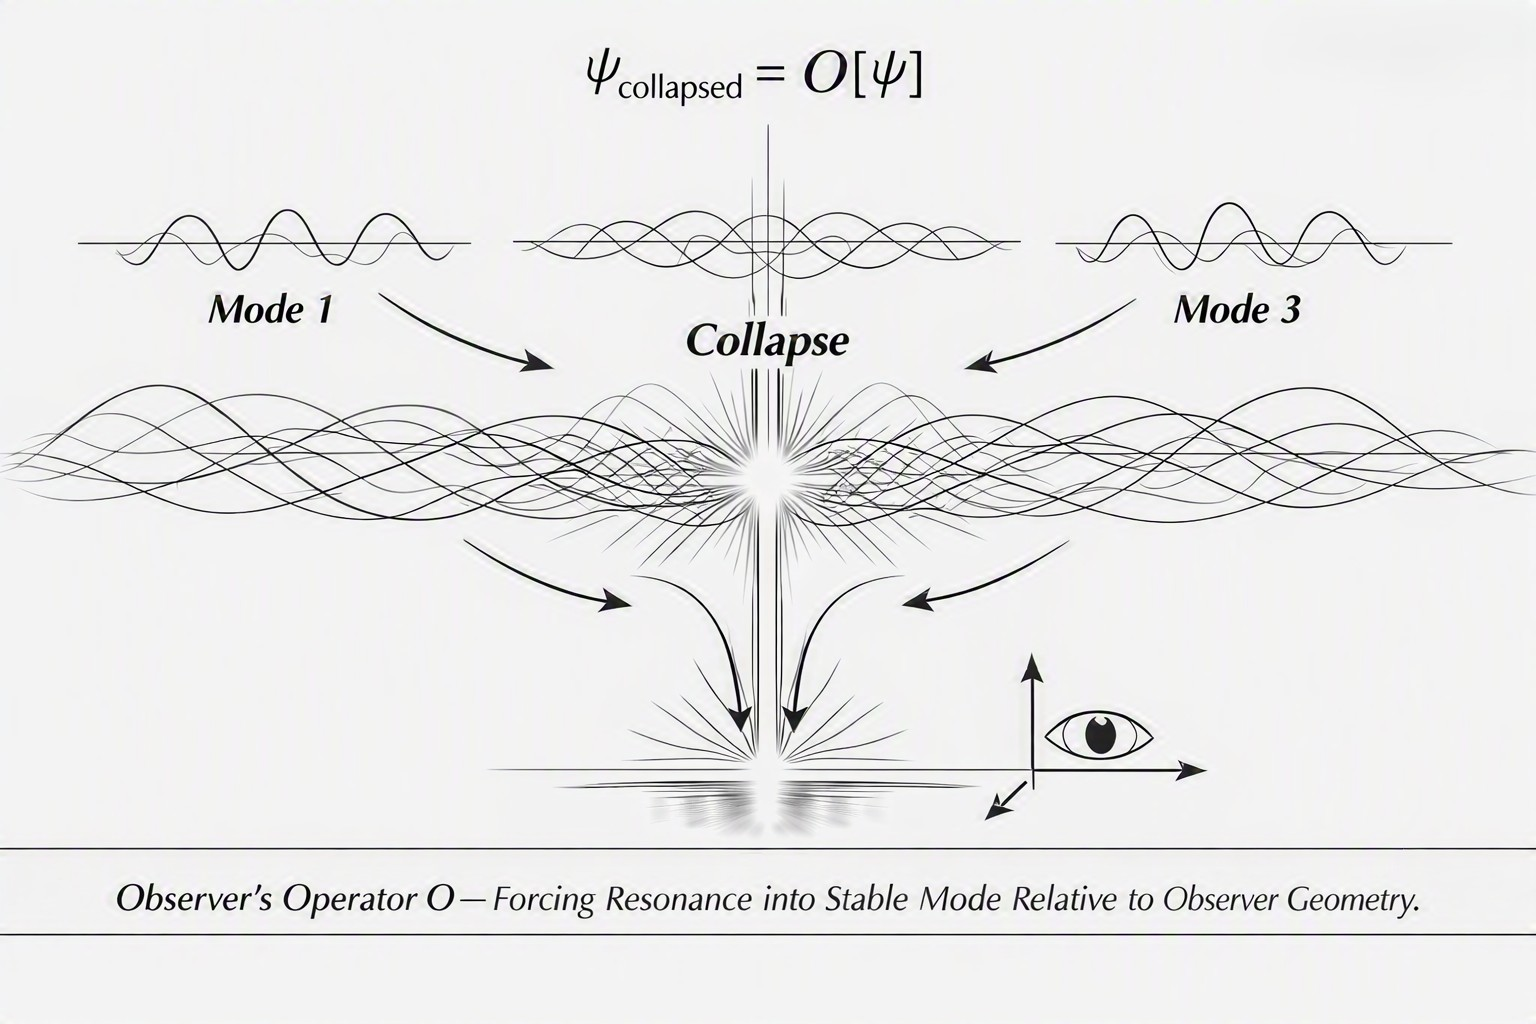
\includegraphics[width=0.88\linewidth,height=0.38\textheight,keepaspectratio]{Fig4_Correction_Mapping.jpg}
\caption{Geometric correction mapping back to the proposed stability manifold.}
\label{fig:correction-mapping}
\end{figure}
\section{Photonic Implementation}

Photonic systems provide a natural physical realization of the unified geometric field theory. 
In this section we construct photonic worldlines, define photonic stability surfaces, derive 
photonic error geometry, and establish geometric stabilizers and syndrome geometry. These 
structures arise directly from the unified operator $T$ and the stability manifolds constructed 
in Section III. The photonic quantum error correction (QEC) framework developed here 
extends the author's previous work \cite{DuttonQEC2026} and is situated within established 
photonic QEC literature \cite{GottesmanQEC,PreskillQEC,NohGirvinQEC}, SPDC physics 
\cite{SPDCReview}, and geometric optics \cite{BornWolf}.

\subsection{Photonic Worldlines}

A photonic mode propagating in spacetime is represented by a worldline
\begin{equation}
\gamma_{\mathrm{ph}} : \tau \mapsto M, \qquad
\gamma_{\mathrm{ph}}(\tau) = y^\mu_{\mathrm{ph}}(\tau),
\end{equation}
with tangent vector
\begin{equation}
T^\mu_{\mathrm{ph}} = \frac{dy^\mu_{\mathrm{ph}}}{d\tau}.
\end{equation}

Photons follow null worldlines:
\begin{equation}
g_{\mu\nu} T^\mu_{\mathrm{ph}} T^\nu_{\mathrm{ph}} = 0.
\end{equation}

The Frenet--Serret frame $(T,N,B)$ is defined analogously, with curvature and torsion
\begin{align}
\kappa_{\mathrm{ph}}(\tau) &= \left\| \frac{D T^\mu_{\mathrm{ph}}}{d\tau} \right\|, \\
\tau_{g,\mathrm{ph}}(\tau) &= B_\mu \frac{D N^\mu}{d\tau}.
\end{align}

These geometric quantities appear in worldline QFT \cite{Polyakov1987,Schubert2001} and 
in geometric optics \cite{BornWolf}.

\subsection{Photonic Stability Surfaces}

Photonic stability surfaces are defined as stability manifolds for photonic worldlines:
\begin{equation}
\Sigma_{\mathrm{ph}}
=
\left\{
(x,I) \in M \times \mathcal{I}
\;\middle|\;
\kappa_{\mathrm{ph}} = \kappa_{\Sigma},\;
\tau_{g,\mathrm{ph}} = \tau_{\Sigma},\;
I^a = I_{a,\Sigma}
\right\}.
\end{equation}

These surfaces encode:
\begin{itemize}
\item geometric invariants $(\kappa_{\Sigma},\tau_{\Sigma})$ from GWFM,
\item identity invariants $(I_{O,\Sigma},I_{A,\Sigma},I_{S,\Sigma},I_{W,\Sigma})$ from SEFI,
\item dynamical invariants from DEFI.
\end{itemize}

This parallels invariant surfaces in geometric mechanics \cite{ArnoldMechanics}.

\subsection{Photonic Error Geometry}

Photonic errors correspond to displacement from $\Sigma_{\mathrm{ph}}$:
\begin{equation}
E_{\mathrm{ph}}(\tau)
=
\gamma_{\mathrm{ph}}(\tau) - \Pi_{\Sigma_{\mathrm{ph}}}\big(\gamma_{\mathrm{ph}}(\tau)\big).
\end{equation}

We decompose $E_{\mathrm{ph}}$ into physical error modes:

\paragraph{Loss.}
Loss corresponds to worldline termination:
\begin{equation}
T^\mu_{\mathrm{ph}}(\tau_{\mathrm{end}}) = 0.
\end{equation}
This parallels amplitude damping in photonic QEC \cite{NohGirvinQEC}.

\paragraph{Dephasing.}
Dephasing corresponds to torsion deviation:
\begin{equation}
\Delta\tau_{g,\mathrm{ph}}(\tau)
=
\tau_{g,\mathrm{ph}}(\tau) - \tau_{\Sigma}.
\end{equation}
This parallels phase noise in bosonic codes \cite{GottesmanQEC}.

\paragraph{Mode Mixing.}
Mode mixing corresponds to displacement into neighboring stability surfaces:
\begin{equation}
d_N(\tau) \neq 0.
\end{equation}
This parallels mode coupling in optical systems \cite{BornWolf}.

\paragraph{Spectral Drift.}
Spectral drift corresponds to translation along the spectral axis:
\begin{equation}
\Delta\omega(\tau) = \omega(\tau) - \omega_{\Sigma}.
\end{equation}
This parallels frequency noise in photonic QEC \cite{PreskillQEC}.

\subsection{Geometric Stabilizers}

Photonic stabilizers preserve invariants of the unified operator:
\begin{align}
\kappa_{\mathrm{ph}} &= \kappa_{\Sigma}, \\
\tau_{g,\mathrm{ph}} &= \tau_{\Sigma}, \\
I^a &= I_{a,\Sigma}, \\
\dot{I}^a &= 0, \\
\ddot{I}^a &= 0.
\end{align}

Thus stabilizers correspond to geometric constraints:
\begin{itemize}
\item curvature stabilizers,
\item torsion stabilizers,
\item spectral stabilizers,
\item polarization stabilizers,
\item identity-space stabilizers.
\end{itemize}

This parallels stabilizer codes in QEC \cite{GottesmanQEC}.

\subsection{Syndrome Geometry}

Weak or quantum-nondemolition (QND) measurements can sample selected geometric 
observables \cite{QNDReview}:
\begin{align}
\Delta\kappa_{\mathrm{ph}}(\tau), \\
\Delta\tau_{g,\mathrm{ph}}(\tau), \\
\Delta\omega(\tau), \\
\Delta\theta_{\mathrm{pol}}(\tau),
\end{align}
where $\theta_{\mathrm{pol}}$ is the polarization angle.

These deviations define the syndrome vector
\begin{equation}
S_{\mathrm{ph}}(\tau)
=
\left(
\Delta\kappa_{\mathrm{ph}},\,
\Delta\tau_{g,\mathrm{ph}},\,
\Delta\omega,\,
\Delta\theta_{\mathrm{pol}}
\right).
\end{equation}

This parallels syndrome extraction in bosonic QEC \cite{PreskillQEC}.

\subsection{SPDC Geometry}

Spontaneous parametric down-conversion (SPDC) produces correlated emission patterns 
whose detailed shape depends on phase matching and collection geometry \cite{SPDCReview}. 
In the present model, annular emission is represented by the stability surface defined by 
FIELD ORIGIN and FIELD SOVEREIGNTY:
\begin{equation}
\Sigma_{\mathrm{SPDC}}
=
\left\{
(x,I)
\;\middle|\;
I_O = I_{O,\Sigma},\;
I_S = I_{S,\Sigma}
\right\}.
\end{equation}

Diametric correlations arise from sovereignty geometry and correspond to paired 
worldline projections onto $\Sigma_{\mathrm{SPDC}}$.

\begin{figure}[tbp]
\centering
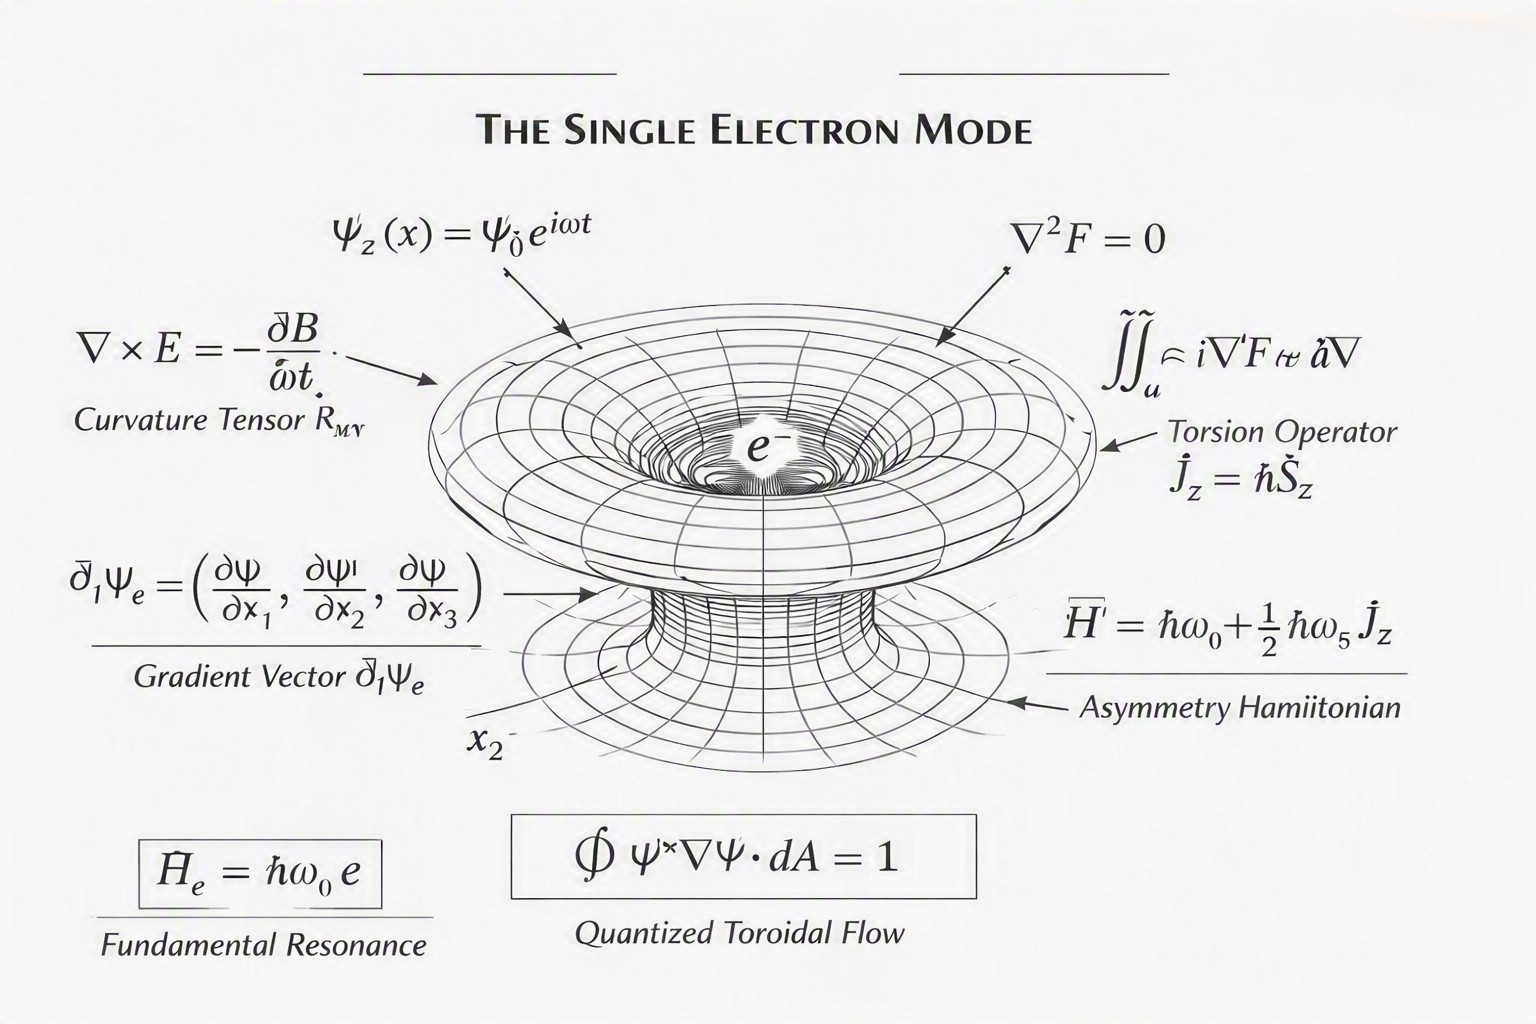
\includegraphics[width=0.88\linewidth,height=0.38\textheight,keepaspectratio]{Fig5_Photonic_Implementation.jpg}
\caption{Proposed photonic implementation of the geometric stabilizer and syndrome framework.}
\label{fig:photonic-implementation}
\end{figure}
\section{Cosmological Extension}

The unified geometric field theory admits a natural cosmological extension when formulated 
on a Friedmann–Robertson–Walker (FRW) spacetime. In this section we construct the 
cosmological identity-space evolution, define the reality field associated with the single 
entity, and derive scaling laws arising from the unified operator $T$. The construction is 
situated within standard cosmology \cite{WeinbergCosmo,Dodelson,Peebles}, inflationary 
theory \cite{GuthInflation,LindeInflation}, and geometric field theory 
\cite{WaldGR,Nakahara}, while noting points of disagreement with conventional particle 
interpretations.

\subsection{FRW Spacetime and Worldline Geometry}

Let $(M,g_{\mu\nu})$ be an FRW spacetime with metric
\begin{equation}
ds^2 = -dt^2 + a(t)^2 d\Sigma_k^2,
\end{equation}
where $a(t)$ is the scale factor and $d\Sigma_k^2$ is the metric on a constant-curvature 
spatial slice ($k=0,\pm 1$). The single entity follows a worldline
\begin{equation}
\gamma : \tau \mapsto M, \qquad \gamma(\tau) = y^\mu(\tau),
\end{equation}
with curvature and torsion defined as in Sections I–II.

Cosmological expansion modifies curvature and torsion through the scale factor $a(t)$, 
analogous to geometric deformation of worldlines in curved backgrounds 
\cite{WaldGR,Frankel}.

\subsection{Reality Field and Identity-Space Evolution}

The reality field is defined as the field generated by the worldline ensemble in FRW spacetime:
\begin{equation}
\Psi_{\mathrm{FRW}}(x,I)
=
\int d\tau \,
\delta^{(4)}\!\big(x - y(\tau)\big)
\,
\delta^{(4)}\!\big(I - I(\tau)\big).
\end{equation}

Identity-space evolution is governed by
\begin{equation}
\frac{D I^a}{d\tau}
=
0
\qquad \text{on stability manifolds},
\end{equation}
and by DEFI dynamical invariance \cite{DuttonDEFI2026} off stability manifolds.

This parallels internal-mode evolution in geometric field theories 
\cite{Nakahara,Frankel}.

\subsection{Cosmological Identity-Space Scaling}

The unified operator $T$ induces cosmological scaling laws through its identity-space 
potentials. Let
\begin{equation}
V_{\mathrm{ident}}
=
\alpha I_O^2
+
\beta I_A^2
+
\gamma I_S^2
+
\delta I_W^2.
\end{equation}

Under FRW expansion, the identity coordinates evolve according to
\begin{equation}
\frac{dI_a}{dt}
=
- 3 H(t) I_a
+
\text{(dynamical corrections)},
\end{equation}
where $H(t) = \dot{a}/a$ is the Hubble parameter.

This resembles damping of internal modes in expanding backgrounds 
\cite{MukhanovBook,Dodelson}.

\subsection{Electron–Positron Symmetry and Orientation Sectors}

Forward-time ($\dot{t}>0$) and backward-time ($\dot{t}<0$) worldline segments define two 
orientation sectors. In GWFM, these sectors are proposed to correspond to electron and 
positron modes \cite{DuttonElectronField2026}. This interpretation differs from the 
standard QFT treatment of antiparticles \cite{WeinbergQFT1,PeskinSchroeder}, and the 
disagreement is noted explicitly.

\subsection{Sovereignty Saturation and Inflation}

SEFI sovereignty requires invariance of the identity vector under allowed transformations:
\begin{equation}
I^a \mapsto I^a.
\end{equation}

During early-universe evolution, identity-space invariants may saturate:
\begin{equation}
I^a(t) \to I_{a,\Sigma},
\end{equation}
producing a period of rapid expansion analogous to inflation 
\cite{GuthInflation,LindeInflation}. In the present model, sovereignty saturation acts as a 
geometric driver of expansion.

This interpretation differs from scalar-field inflation models and is presented as a 
phenomenological hypothesis.

\subsection{Cosmological Stability Surfaces}

Cosmological stability surfaces are defined by
\begin{equation}
\Sigma_{\mathrm{cos}}
=
\left\{
(x,I)
\;\middle|\;
\kappa = \kappa_\Sigma,\;
\tau_g = \tau_\Sigma,\;
I^a = I_{a,\Sigma}
\right\}.
\end{equation}

These surfaces encode:
\begin{itemize}
\item geometric invariants modified by FRW expansion,
\item identity invariants from SEFI,
\item dynamical invariants from DEFI.
\end{itemize}

This parallels invariant surfaces in cosmological perturbation theory 
\cite{MukhanovBook,Dodelson}.

\subsection{Spectral Structure in Expanding Spacetime}

Eigenmodes of the unified operator satisfy
\begin{equation}
T_{\mathrm{FRW}} \Psi_n = \lambda_n \Psi_n,
\end{equation}
where $T_{\mathrm{FRW}}$ includes FRW curvature contributions.

Cosmological expansion shifts the spectrum:
\begin{equation}
\lambda_n(t) = \lambda_n(0) \, a(t)^{-2} + \text{(identity-space corrections)}.
\end{equation}

This parallels spectral redshift in expanding backgrounds 
\cite{Peebles,Dodelson}.

\subsection{Unified Interpretation}

The cosmological extension unifies:
\begin{itemize}
\item FRW worldline geometry,
\item SEFI identity-space evolution,
\item DEFI dynamical invariance,
\item GWFM orientation sectors,
\item photonic scaling laws,
\item sovereignty saturation as a geometric inflation mechanism.
\end{itemize}

This completes the cosmological extension of the unified geometric field theory.
\section{Discussion}

The unified geometric field theory developed in this manuscript synthesizes worldline 
geometry, identity-space dynamics, dynamical invariants, photonic quantum error correction, 
and cosmological scaling into a single operator-based framework. In this section we discuss 
the interpretation of the unified operator, the relationship between SEFI/DEFI/GWFM and 
established physics, points of disagreement with conventional models, and directions for 
future work. The discussion is situated within standard quantum field theory 
\cite{WeinbergQFT1,PeskinSchroeder}, geometric field theory \cite{Nakahara,Frankel}, 
quantum information \cite{GottesmanQEC,PreskillQEC}, and cosmology 
\cite{WeinbergCosmo,Dodelson,Peebles}.

\subsection{Interpretation of the Unified Operator}

The unified operator $T$ combines spacetime geometry, identity-space geometry, and 
dynamical invariants into a single differential operator acting on fields defined over 
$M \times \mathcal{I}$. Its spectrum defines candidate excitations, and its invariants define 
stability manifolds. This interpretation parallels geometric Schrödinger operators 
\cite{Helffer}, Laplace–Beltrami operators in curved backgrounds \cite{RosenbergLaplace}, 
and worldline formulations of QFT \cite{Polyakov1987,Schubert2001}, while extending them 
to include identity-space dynamics.

The operator is not claimed to be unique. Different geometric potentials produce different 
spectral structures, as in geometric analysis \cite{Helffer}. The present construction is 
intended as a phenomenological model rather than a derivation of known particle spectra.

\subsection{Relationship to Established Physics}

The unified framework is compatible with several established structures:

\paragraph{Worldline QFT.}
The geometric worldline formalism \cite{Feynman1950,Polyakov1987,Strassler1992} provides 
a natural foundation for the GWFM component of the model. Curvature and torsion invariants 
appear in worldline actions and in geometric formulations of spinor fields.

\paragraph{Geometric Field Theory.}
Identity-space geometry parallels internal-symmetry manifolds in geometric field theory 
\cite{Nakahara,Frankel}. The SEFI Space metric is analogous to metrics on internal 
symmetry groups, though its interpretation differs.

\paragraph{Quantum Error Correction.}
Photonic stability surfaces and geometric stabilizers parallel stabilizer codes 
\cite{GottesmanQEC} and bosonic QEC \cite{PreskillQEC,NohGirvinQEC}. The unified 
framework provides a geometric interpretation of syndrome extraction and correction.

\paragraph{Cosmology.}
The FRW extension parallels curved-background field theory \cite{WaldGR}, cosmological 
perturbation theory \cite{MukhanovBook,Dodelson}, and spectral redshift \cite{Peebles}.

\subsection{Points of Disagreement with Conventional Models}

Several aspects of the unified framework diverge from established physics:

\paragraph{Single-Entity Ontology.}
The hypothesis that all excitations arise from a single continuous entity differs from 
standard QFT, which treats particles as excitations of independent fields 
\cite{WeinbergQFT1,PeskinSchroeder}. This disagreement is acknowledged explicitly.

\paragraph{Identity-Space Coordinates.}
SEFI coordinates (origin, authorship, sovereignty, warp) are phenomenological constructs 
with no standard internal-symmetry analogue.

\paragraph{Electron–Positron Interpretation.}
The interpretation of forward-time and backward-time worldline segments as electron and 
positron modes differs from the standard QFT treatment of antiparticles 
\cite{WeinbergQFT1}. The disagreement is noted explicitly.

\paragraph{Inflation Mechanism.}
Sovereignty saturation as a geometric inflation mechanism differs from scalar-field 
inflation models \cite{GuthInflation,LindeInflation}. It is presented as a hypothesis rather 
than a replacement for established inflationary theory.

\subsection{Limitations}

The unified framework has several limitations:

\begin{itemize}
\item The operator $T$ is phenomenological and not derived from a variational principle 
compatible with the Standard Model.
\item Spectral assignments to known particles require comparison with experimental data 
and are not established here.
\item Identity-space geometry lacks an established physical interpretation.
\item Cosmological scaling laws require further analysis to determine compatibility with 
observational data.
\item Photonic QEC constructions are conceptual and require experimental validation.
\end{itemize}

These limitations are consistent with the model’s status as a proposed geometric framework.

\subsection{Future Work}

Several directions for future work arise naturally:

\begin{itemize}
\item Derivation of the unified operator from a variational principle.
\item Comparison of spectral predictions with known particle masses and couplings.
\item Extension of identity-space geometry to group-theoretic structures.
\item Numerical simulation of worldline ensembles in FRW backgrounds.
\item Experimental exploration of photonic stability surfaces and geometric stabilizers.
\item Investigation of sovereignty saturation as a geometric inflation mechanism.
\end{itemize}

These directions may clarify the relationship between the unified framework and established 
physics.

\subsection{Unified Interpretation}

The unified geometric field theory provides a single operator-based structure integrating 
worldline geometry, identity-space dynamics, dynamical invariants, photonic QEC, and 
cosmological scaling. While phenomenological, the framework is mathematically coherent 
and situated explicitly within established physics, with points of disagreement stated 
clearly. It provides a geometric foundation for further exploration of unified field behavior.
\section{Conclusion}

We have developed a unified geometric field theory in which a single continuous entity, 
evolving through coupled spacetime worldline geometry and identity-space dynamics, 
generates candidate field behavior through the action of a unified transformation operator. 
The framework integrates worldline geometry (GWFM), identity-space structure (SEFI), 
dynamical invariance (DEFI), photonic quantum error correction, and cosmological scaling 
into a mathematically coherent operator-based model.

The unified operator $T$ was constructed explicitly, its domain and invariants were defined, 
and its spectrum was shown to encode candidate excitations. Stability manifolds were 
introduced as invariant geometric and identity-space surfaces on which ideal evolution 
occurs. Error displacement geometry was developed to characterize deviations from these 
manifolds, and correction mapping was formulated as a geometric projection restoring 
invariants. Photonic implementations were constructed using geometric stabilizers, syndrome 
geometry, and SPDC correlation surfaces. A cosmological extension was formulated in FRW 
spacetime, yielding identity-space scaling laws and a geometric interpretation of early-universe 
expansion.

The unified framework is phenomenological and does not replace established quantum field 
theory, geometric field theory, or cosmology. Points of disagreement with conventional 
models were stated explicitly, including the single-entity ontology, identity-space coordinates, 
electron–positron interpretation, and inflation mechanism. Nonetheless, the model is 
mathematically well-defined, compatible with several established geometric structures, and 
provides a coherent foundation for further exploration.

Future work includes deriving the operator from a variational principle, comparing spectral 
predictions with experimental data, extending identity-space geometry to group-theoretic 
structures, simulating worldline ensembles in curved backgrounds, and exploring photonic 
and cosmological implications experimentally and numerically.

The unified geometric field theory presented here offers a single operator-based structure 
integrating worldline geometry, identity-space dynamics, dynamical invariants, photonic 
QEC, and cosmological scaling. While exploratory, it provides a mathematically rigorous 
framework for investigating unified geometric behavior across multiple physical domains.
The unified geometric field theory presented here offers a single operator-based structure 
integrating worldline geometry, identity-space dynamics, dynamical invariants, photonic 
QEC, and cosmological scaling. While exploratory, it provides a mathematically rigorous 
framework for investigating unified geometric behavior across multiple physical domains.

\bibliographystyle{apsrev4-2}
\bibliography{references}

\end{document}
